\chapter{Solution}
\label{cha:solution}

Here we gonna talk about the solution, its organization and components. Every component will have a detailed explanation.

\section{Organization} % (fold)
\label{sec:organization}

The process of generating an API based on a xsd file contents is complex, so in order to simplify it it was divided into two smaller projects, each one with a given goal and responsibilities. The two main responsibilities in this process are parsing the information from the xsd file and generating the API based on that same parsed information.

\section{Parsing} % (fold)
\label{sec:parsing}

%TODO Review all this text.

The parser will have the responsibility to read the XML schema element tree and extract the needed information in order to generate the respective classes. The result of the execution of this component should be a list of elements, each element representing a class that should be created and containing all the information needed for the creation.

\subsection{Document Object Model} % (fold)
\label{sec:dom}

What is DOM? Why does its usage applies in this project? If DOM exists why does this project implements a XsdParser? Are there any alternatives to DOM, and if so, why was DOM chosen?

\section{Code Generation} % (fold)
\label{sec:codegeneration}

%TODO Review all this text.

The class generator will have the responsibility of generating classes based on the information received from the Parser. The class generator should request the parsing of a XML schema file and based on the Parser result, create the classes accordingly. Apart from that the generator should also create an infrastructure that will help the usage of the the resulting API. 

\noindent
To achieve the generation of the classes a tool named ASM will be used. This tool allows the manipulation of byte codes, allowing the generation of classes, methods and fields. 

\newpage

\subsection{Supporting Infrastructure}

The generated code will be supported by an infrastructure that mimics the syntax of XML schema files. The supporting infrastructure is shown in \ref{Infrastructure}.

\begin{figure}[h]
	\centering
	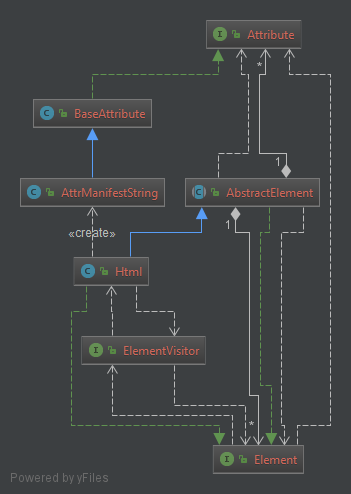
\includegraphics[width=0.65\textwidth]{infrastructure}
	\caption{Supporting Infrastructure}
	\label{Infrastructure}
\end{figure}

\noindent
All the generated APIs will have this classes which are independent of the contents of the parsed file. This infrastructure will then be extended by different type of classes, divided in four groups.

\textbf{Elements}

The elements are a group of classes that will be generated based in the existing xsd:elements. All these classes will extend AbstractElement. Each element will also contain the specific element code, which can include addition of elements, attributes or implementing group and element interfaces.

\textbf{Attributes}

The attributes are a group of classes that will be generated based in the existing xsd:attributes. All these classes will extend AbstractAttribute. Each attribute will have a type, that indicates the type of the value of the said attribute. Attributes will also enforce restrictions to their value if there are any explicitly described in the XML schema file.

\textbf{Group Interface}

The group interfaces are an addiction that represent the xsd:attributegroups. In the XML schema these attributegroups indicate that a given element is allowed to have the said attributes, in the generated code the respective interfaces allow the addiction of all the attributes present in the said group to the element attributes.

\textbf{Element Interface}

The element interfaces are similar to the group interfaces, the difference being that element interfaces allow the addiction of other elements as children of the current element. 

\textbf{Visitors}

In order to the generated API allow manipulation by the client all the generated elements implement the Visitor pattern, therefore the client of the API can implement its own Visitor class and specify the behavior of the visit methods.

\subsection{ASM} % (fold)
\label{sec:asm}

What is ASM? Why is it important in this project? Are there any alternatives to ASM? If so why was ASM chosen?

\section{Client} % (fold)
\label{sec:client}

Some stuff here.

\section{HtmlFlow}
\label{sec:htmlflow}

More stuff here.
